% select subfiles base file
\documentclass[TGAI_Laborbericht.tex]{subfiles}
\begin{document}

\chapter{Versuch 4}
\label{chap:VERSUCH_4}

\section{Fragestellung, Messprinzip, Aufbau, Messmittel}
\label{chap:VERSUCH_4_FRAGESTELLUNG}
Wir sollen nun das Dunkelbild auf hot und stuck pixel sowie das Weißbild auf dead pixel untersuchen und diese auf den bildern kenntlich machen. Außerdem wird nun das ursprüngliche Graukeil Bild mithilfe des Dunkel und Weißbildes korrigiert. Anschließend werden die Mittelwerte und Standartabweichungen des ursprünglichen Bildes und des korrigierten Bildes gegenübergestellt.

\section{Messwerte}
\label{chap:VERSUCH_4_MESSWERTE}
Jetzt überprüfen wir das Dunkelbild auf stuck und hot pixel und das Weißbild auf dead pixel.
\begin{figure}[H]
	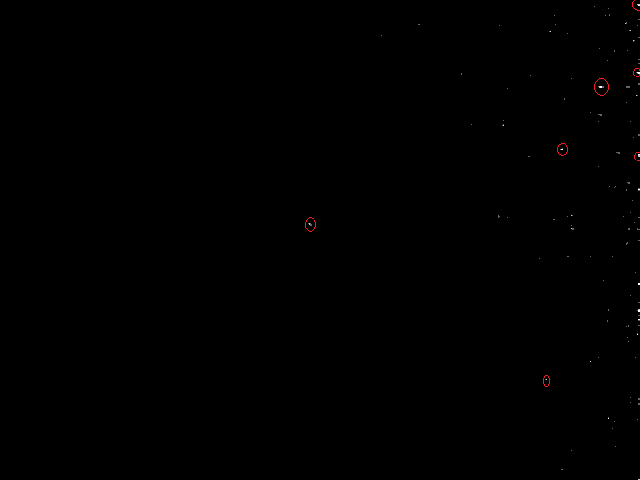
\includegraphics[width=0.7\textwidth]{media/stuck&hotpixel.png}
	\caption{stuck und hot pixel}
	\label{fig:stuck und hot pixel}
\end{figure}

\begin{figure}[H]
	
\includegraphics[width=0.7\textwidth]{media/Weissbild.png}
	\caption{Weissbild}
	\label{fig:Weissbild}
\end{figure}

\section{Auswertung}
\label{chap:VERSUCH_4_AUSWERTUNG}
Beim Dunkelbild lassen sich wie man in der Abbildung erkennen kann, einige hot bzw. stuck pixel ausfindig machen. Im Weissbild hingegen ließen sich keine dead pixel finden.
Desweiteren werden jetzt für das korrigierte Bild die Mittelwerte und Standardabweichtungen für die einzelnen Graustufen berechnet. 

\begin{tabular}{|c|c|c|c|c|}
\hline 
Versuch1: & • & • & Verbesserung: & • \\ 
\hline 
• & Mittelwerte & Standardabweichung & Mittelwerte Neu & Standardabweichung Neu \\ 
\hline 
Weiß & 212.999089506 & 4.96548417796 & 224.655131173 & 3.4856729337 \\ 
\hline 
Hellgrau & 187.409228395 & 6.13117423931 & 190.358688272 & 4.31304726086 \\ 
\hline 
Grau & 137.798001543 & 4.78215632893 & 135.730864198 & 4.87338968593 \\ 
\hline 
Dunkelgrau & 82.7268364198 & 3.67189805988 & 80.9926388889 & 4.92684835396 \\ 
\hline 
Schwarz & 42.7226466049 & 6.93616814165 & 41.8664660494 & 7.196487838 \\ 
\hline 
\end{tabular} 

\section{Interpretation}
\label{chap:VERSUCH_4_INTERPRETATION}

Da wir jetzt die neuen Mittelwerte und Standardabweichungen haben, können wir diese mit den Werten aus Versuch 1 vergleichen. Wir kommen zu dem Schluss, dass es sowohl in den Mittelwerten als auch in der Standardabweichung leichte Veränderungen gab. Aufgrund unserer Messergebnisse lässt sich jedoch keine eindeutige Verbesserung nachweisen.

\end{document}